\begin{figure}
    \centering

    % Parameters
    \def\nodessep{1}
    \def\n{10} % Number of nodes (each part)
    \def\cellsize{0.5} %set as 5 divided by \n

    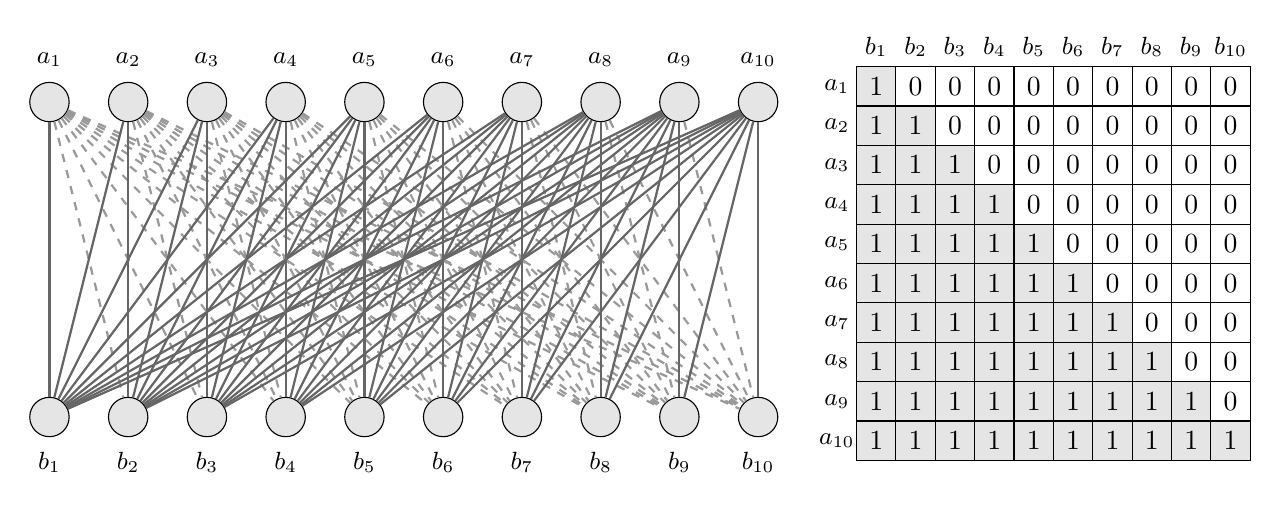
\begin{tikzpicture}[
        vertex/.style={circle, draw, fill=gray!20, minimum size=5mm, inner sep=1pt},
        label_a/.style={above=2pt, font=\small},
        label_b/.style={below=2pt, font=\small},
        node distance=1.5cm,
        solid edge/.style={draw, thick, black!60},
        dashed edge/.style={draw, dashed, thick, black!40},
        matrix cell/.style={draw, minimum size=\cellsize cm, inner sep=0pt},
        matrix label/.style={font=\small, anchor=center}
    ]

    % Graph nodes (top and bottom)
    % Top part vertices (a_i)
    \foreach \i in {1,...,\n} {
        \node[vertex] (a\i) at (\i*\nodessep, 0) {};
        \node[label_a] at (a\i.north) {$a_{\i}$};
    }

    % Bottom part vertices (b_j)
    \foreach \j in {1,...,\n} {
        \node[vertex] (b\j) at (\j*\nodessep, -4) {};
        \node[label_b] at (b\j.south) {$b_{\j}$};
    }

    % Draw edges
    \foreach \i in {1,...,\n} {
        \foreach \j in {1,...,\n} {
            \ifnum\i<\j
                \draw[dashed edge] (a\i) -- (b\j);
            \else
                \draw[solid edge] (a\i) -- (b\j);
            \fi
        }
    }

    % Adjacency Matrix
    \begin{scope}[xshift=2cm+\n*\nodessep cm]

    % Matrix labels
    \foreach \i in {1,...,\n} {
        \node[matrix label] at (-1 + \i*\cellsize, 0.7) {$b_{\i}$};
        \node[matrix label] at (-1, 0.7 -\i*\cellsize) {$a_{\i}$};
    }

    % Draw the matrix cells and fill based on adjacency
    \foreach \i in {1,...,\n} {
        \foreach \j in {1,...,\n} {
            \pgfmathsetmacro{\xcoord}{\j*\cellsize}
            \pgfmathsetmacro{\ycoord}{-\i*\cellsize}
            \ifnum\i<\j
                \node[matrix cell] at (-1 + \xcoord, 0.7 + \ycoord) {0};
            \else
                \node[matrix cell, fill=gray!20] at (-1 + \xcoord, 0.7 + \ycoord) {1};
            \fi
        }
    }

    \end{scope}

    \end{tikzpicture}
    \caption{
        A half-graph with 2 × 10 vertices.
        \emph{On the left}, solid lines show adjacent vertices, and dashed lines show non-adjacent vertices.
        Pairs of vertices without a line may or may not be connected.
        \emph{On the right} is the corresponding adjacency matrix.
    }
    \label{fig:half_graph}
\end{figure}